\documentclass[a4paper,11pt]{article}

% Padding Requirements
\usepackage[a4paper, margin=1in]{geometry}
% used for double spacing
\usepackage{setspace}
\doublespacing
% Used for images
\usepackage{graphicx}
\usepackage{float}
\graphicspath{{/Users/sloth_mini/Documents/4.1/dissertation/images/}}
% Used for bibliography
\usepackage[style=ieee, sorting=none, backend=biber]{biblatex}
\renewcommand{\bibfont}{\small}
% For math notation
\usepackage{amsmath}
\newcommand{\setA}{\{A\}}
\newcommand{\setB}{\{B\}}
\newcommand{\abrule}{\setA\rightarrow\setB}

\addbibresource{references.bib}

% Do we need a table of contents? I don't think so.
\begin{document}
\title{Deliverable 1: Final Year Dissertation}
\author{
	Sahil Pattni\\ 
	BSc. Computer Science (Honours)\\\\
	Supervisor: Neamat El Gayar
	}
\date{\today}
\maketitle
\pagenumbering{arabic}
\newpage
\section*{Declaration} 
I, Sahil Manojkumar Pattni, confirm that this work submitted for assessment is my own and is expressed in my own words. Any uses made within it of the works of other authors in any form (e.g., ideas, equations, figures, text, tables, programs) are properly acknowledged at any point of their use. A list of the references employed is included. 
\\
Signed: Sahil Manojkumar Pattni\\
Date: \today

\section*{Abstract}
In this digital age, data is being generated at an exponential rate, with data analytics being used by corporations and small businesses alike to produce insights, reduce costs, optimize operations and increase profits.  Generating association rules allow us to find non-intuitive associations that bring new insights to the management, allowing them to leverage this information to maximize their profits. A prime example would be the \textit{'Beers and Diapers'} case \cite{beers_diapers}, where a company looked at their point-of-sale data and found a strong association between beers and diapers being co-purchased, which seems rather unintuitive.\\
In this study, we will extract a minimum spanning tree (MST) from a data set using machine learning techniques. We will then use this minimum spanning tree to segment products together,  and produce association rules and extract the most interesting ones. The resulting ruleset will be compared to rules generated by the established Apriori Algorithm \cite{apriori}, which is the foundation of association rule mining.  Additionally, we will study how the grouping of the MST compares to clustering algorithms, and how the structure of our MST would change before and after promotional events, leading to insights that may help the management in such firms make better informed decisions about the type of promotions they would like to run.

\newpage
\tableofcontents

\newpage
\section{Introduction}
\subsection{Context}
For business which deal with the sale of a heterogeneous physical assets - such as groceries, hypermarkets and select retail outlets - operations such as inventory management and product placement play an instrumental role in determining the business' financial success. These involve asking questions such as:
\begin{itemize}
\item Which products should be placed at the entrance of the store? Which should be placed closer to the exit?
\item Which products will benefit the most by being placed at eye-level?
\item Which products should be placed next to each other to maximize the purchase volume?
\end{itemize}
One way to find optimal solutions for such questions is to employ the use of Association Rule Mining (also known as Market Basket Analysis). This set of techniques assess frequent itemsets (e.g. from sales data) and generate association rules between products. Several algorithms and techniques exist for association rule mining, such as the Apriori Algorithm and FP-Growth \cite{fp_growth}. One problem with these algorithms is that they tend to generate an enormous amount of rules, of which many of the rules themselves are large This makes it grossly inconvenient for the end-user to retrieve any actionable information from the results.\\
What we will do is construct a network of products - where each vertice represents a product or product category, and an edge between two vertices represents the simultaneous occurrence of the the two products. The result is a graph (i.e. a network), whose architecture is visually informative of the products and their associations.  The insights that can be gained from the MST can help the management of the mentioned businesses to maximize their profit.

\subsection{Aims}
The aim of this study is to study the effectiveness of a minimum spanning tree as a market basket analysis tool - from product clustering to association rule mining.  Additionally, we will determine how the architecture of the MST will change during and after large events such as promotions. The model will be tested on a relatively large dataset of sales data.

\subsection{Objectives}
The research objectives for this project have been laid out below, in the order that they will be carried out.
\begin{enumerate}
\item Acquire a suitable dataset upon which the MST can be constructed.

\item \label{optimal} Explore and evaluate MST extraction algorithms.
\\(While Prim's \cite{prims}\cite{prims_og} and Kruskal's \cite{kruskal} algorithms are the most commonly used methods to extract the MST from a graph, research has been conducted on more efficient ways to extract the MST using machine learning techniques such as Artificial Neural Networks and K-Nearest-Neighbors, and these will be discussed in the literature review (see Section \ref{related-work}).

\item Generate an undirected graph $G(E,V)$ where the edges $E$ are the correlation values between the product vertices.

\item Extract a minimum spanning tree from this graph using the technique determined in step \ref{optimal}. 

\item Analyze this MST and use its architecture to determine product clusters and generate association rules.

\item Generate association rules using the Apriori and FP-Growth algorithm and compare them in both their time complexity and their \textit{'interestingness'} (i.e. the unintuitive rules they generate).

\item Validate the product grouping present in the MST against a clustering algorithm (e.g.  such as the K-Means algorithm).
\end{enumerate}

\newpage
\section{Background}
\subsection{Core Concepts} % TODO: Maybe change title?
\subsubsection{Graphs}
\begin{figure}[H]
\centering
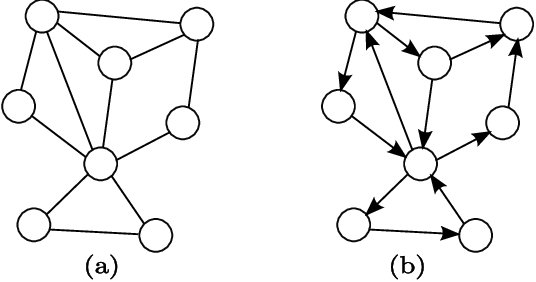
\includegraphics[scale=1.5]{graph-example}
\caption{Undirected and Directed Graphs}
\label{fig:graph.example}
\end{figure}
In discrete mathematics and more specifically - graph theory, a graph is a data structure that contains a set of nodes (i.e. vertices) connected by lines (i.e. edges).  These edges may be directed - such as in Figure \ref{fig:graph.example}:(a), or undirected - such as in Figure \ref{fig:graph.example}:(b). A graph $G$ with a set of vertices $V$ and a set of edges $E$ can be represented via the notation $G = (V,E)$. For the purposes of our research, we will be focusing on undirected graphs, where the weight between two vertices is the same in both directions.
\subsubsection{Minimum Spanning Trees}
Given an undirected $G = (E,V)$,  a \textit{spanning tree} can be described as a subgraph that is a tree which includes all the vertices $V$ of $G$ with the minimum number of edges required. A \textit{minimum spanning tree} (MST) is the spanning tree with the smallest sum of edge weights.  This means that if the graph has $n$ vertices, each spanning tree - including the minimum spanning tree - will have $n-1$ edges.
\newpage
\subsubsection{Market Basket Analysis and Apriori Rule}
\label{mba_define}
Market Basket Analysis (MBA), also known as Affinity Analysis, is a data mining and analysis technique that identifies co-occurrence patterns between products purchased together, and produces association rules for these products as such: $\abrule$ which implies a strong relationship between the purchase of product $A$ and product $B$. In the case of our \textit{Beers and Pampers} example in \cite{beers_diapers}, the association rule could be represented as $\{Beers\} \rightarrow \{Pampers\}$. The contents of a purchase basket (i.e. the contents of a customer's basket when they check out) is called a \textit{itemset}, which - as the name suggests - is a set of all the items in the basket.  For example, if a customer had bought detergent, bread and soda, the itemset would be $\{\textit{bread, detergent, soda}\}$. Association rules are generated by looking at different combinations of the itemset (e.g. $\{\textit{bread, soda}\}\rightarrow\{\textit{detergent}\}$ and $\{\textit{soda}\}\rightarrow\{\textit{bread}\}$). 
The equation \cite{num_rules} to calculate the number of rules for an itemset of length $d$ is as follows :\\
\begin{equation}
\textit{number of rules} = \sum\limits_{k=1}^{d-1} \left(\binom{d}{k} \times \sum\limits_{j=1}^{d-k}\binom{d-k}{j}  \right)
\label{eq:numrules}
\end{equation}
Analyzing the equation, it becomes apparent that the problem with association rule generation from itemsets is that the number of rules produced grows exponentially with the size of the itemset, as we can see in Figure \ref{fig:numrules}, using Equation \ref{eq:numrules}.  
\begin{figure}[H]
\centering
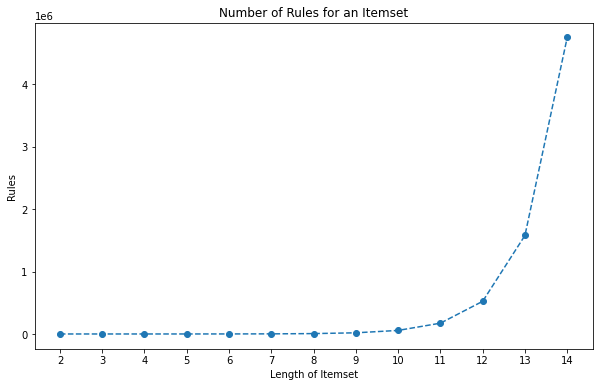
\includegraphics[scale=0.6]{numrules}
\caption{Number of Association Rules for an Itemset}
\label{fig:numrules}
\end{figure}
Clearly, checking all itemsets in a database would be computationally expensive, and so we only look at \textit{frequent itemsets} - itemsets that have a support value above a minimum threshold $\textit{min}_{\textit{support}}$. Even so, checking each itemset's support score via brute force is unacceptably time consuming, therefore we can optimize the search for frequent itemsets using the Apriori Principle \cite{mine} which states that \textit{all subsets of a frequent itemset must be frequent}. To understand how the Apriori Principle can be applied here, we first look at three key metrics:
\\\textbf{Support}\\
The support of a set of products is the fraction of transactions in which these set of products are present. For example,  for a list of transactions $T$, for the product $X$ where $T(X)$ denotes that the set of transactions in which X was present:
\[
\textit{support}(\{A\}) = \frac{T(A)}{T}
\]
and similarly, 
\[
\textit{support}(\abrule) = \frac{T(A,B)}{T}
\]
denotes the support for the rule $\abrule$. We can prune rules with a low support as they indicate a rule does not occur enough to draw any reasonable conclusions from.
\\\textbf{Confidence}\\
Confidence is the measure of how likely a product will be in a basket given that another product is in it. That is to say,  the confidence of a rule $\abrule$ is the conditional probability that $\setB$ occurs in the basket given that $\setA$ is present. The confidence of a rule can be denoted as:
\[
\textit{confidence}(\abrule) = \frac{T(A, B)}{T(A)} \equiv \frac{\textit{support}(\abrule)}{\textit{support}(\setA)}
\]
\\\textbf{Lift}\\
The lift of a rule $\abrule$ is the rise (i.e. \textbf{lift}) that $\setA$ gives to our $\textit{confidence}(\abrule)$.
\[
\textit{lift}(\abrule) = \frac{confidence(\abrule)}{support(\setB)}
\]
To make this easier to understand, imagine that $\textit{confidence}(\abrule)=0.5$, and $\textit{support}(\setB)=0.4.$ This means that the presence of $\setA$ increases the probability of $\setB$ being in the same basket by $25\%$ ($\frac{0.5}{0.4}=1.25$), therefore providing us with a lift value of 1.25.  A lift value below 1 would indicate that the occurrence of $\setA$ in a basket decreases the likelihood of $\setB$ occurring in the same basket (i.e. a low product association).
\\
As we established above,  the Apriori Principle states that all subsets of a frequent itemset must be frequent.  The Apriori Principle is a result of the \textit{anti-monotone property of support} \cite{anti_monotone}, which means $\{A,B,C\}$, $\textit{support}(\{A,B\}) \geq \textit{support}(\{A,B,C\})$.  We can use this to prune the frequent itemsets much more efficiently, because if $support(\{A,B\}) < \textit{min}_{\textit{support}}$, then any itemset containing the set $\{A,B\}$ will also fall below $\textit{min}_{\textit{support}}$. Once the frequent itemsets have been pruned,  association rules can be generated from the remaining itemsets.  The resulting association rules can be even further pruned by removing those that fall below a confidence threshold $\textit{min}_{\textit{confidence}}$.  Finally, the remaining rules can be ranked according to their  lift to find the rules with the highest associations.  

\subsection{Related Work}
\label{related-work}
\textbf{R. Aggarwal et al.} \cite{mine} proposed a novel algorithm to generate all statistically significant association rules between items in a database, laying the foundations for association rule mining.  Given a set of items $I = I_1, I_2, I_3,...I_m$, the authors define an association rule to be of the form $X \rightarrow I_j$ where X is a set of items such that $X \in I, I_j \notin X$.  The hypothetical database stated was a list of transactions, $T$, where each transaction $t$ was a binary vector of length $m$, representing a basket purchase, where $t[k] = 1$ if $I_k$ been purchased in that basket.  The authors stated that their methodology for association rule mining could be split into two steps: the generation of candidate itemsets, and the generation of statistically significant association rules from these itemsets. \\
To address the first subproblem, the authors provided the pseudo-code for their candidate itemset generation,  where all itemsets possible were generated from tuples (samples) from the database,  and those itemsets whose support score\footnote{see: Section \ref{mba_define}} is above the minimum support threshold are considered candidates (called \textit{large itemsets}).  Since a brute-force check would be sub-optimal  (the authors note this could take up to $2^m$ passes of the database),  the authors devised a methodology to check for candidate itemsets where on the $k^{th}$ pass of the database, they would only check itemsets of length $k$, to see if they satisfied the support constraint. On the $(k+1)^{th}$ pass, they need only check those itemsets that are 1-extensions (i.e.  itemsets extended by exactly one item) of the \textit{large itemsets} found in the previous pass. This is because of what would later be known as the \textit{Apriori Principle}, where if an itemset $Y$ is \textit{large}, then all subsets of $Y$ must also be \textit{large}. Therefore, if they found the itemset $\{A,B\}$ was \textit{small} (i.e. did not satisfy the support constraint), then sets containing $\{A,B\}$ (e.g. $\{A,B, C\}, \{A,B, D\}, \{A,B, C, D\}$) would also be small, and need not be checked. This means, however, that if an itemset $I$ is \textit{large}, then another pass over the dataset would be required to check the support of the subsets of $I$. To avoid this, the authors devised a measure to calculate the expected support, $\bar{s}$, of an itemset,  and use this to measure the support of itemsets $I = (X + I_j)$ not only where $I$ is expected to be large, but also where $X+I_j$ is expected to be small but $X$ is expected to be large, further helping them prune the number of itemsets to check.  The authors proceed to define a method that allows the algorithm to be more memory efficient\footnote{This may no longer be required due to the advances in computational speed, capacity and efficiency in the the 27 years since this paper was written.}. The authors also defined method to further prune itemsets from the search, namely \textit{remaining tuples optimization} and \textit{pruning function optimization}.\\
To address the second subprobem,  the authors proposed the following methodology: for each large itemset $Y = I_1, I_2,...I_k, k\geq 2$ from the set of non-pruned large itemsets, generate a set of association rules of form $X \rightarrow I_j$ such that the consequent is $I_j$ and the antecedent (i.e. the precedent set in the rule) is a subset $X$ of $Y$ such that $X$ is of length $k-1$ and $I_j \notin X$. Therefore, each large itemset will produce $k$ rules. From the generated rules, the authors discarded those rules whose confidence scores\footnote{see: Section \ref{mba_define}} fell below the minimum confidence threshold $c$.\\
The authors tested their methodology on a sales dataset with $46,783$ transactions,  with $63$ \textit{items} (in this case, the department from which the customer bought an item). They used a configuration of a minimum support threshold of $1\%$ and a minimum confidence threshold of $50\%$. The rules produced seemed to follow with general intuition, such as:\\
$\{\text{Auto Accessories, Tires}\} \rightarrow \{\text{Automotive Services}\} $\\
Furthermore, the authors assessed the accuracy of their expectation method, by measuring the ratio of correctly estimated itemsets for both small and large, against various values for the minimum support threshold, and visualizing the result. To isolate the effect of their expectation method, they disabled their pruning optimization functions. They were able to conclude that their estimation accuracy was satisfactory, as their accuracy was above 98\% for support thresholds except the first, where it was 96\%.  The authors also tested the effectiveness of their pruning optimization functions, namely the \textit{remaining tuples} and the \textit{pruning function} optimization functions, against multiple minimum support threshold values. They were able to conclude that their pruning efficiency increased as the support threshold increased.
\\\\
% MAIN MST PAPER
\textbf{M. A. Valle et al.} \cite{mst_paper} proposed a novel methodology to study the structure and behavior of consumer market baskets from the topology of a minimum spanning tree which represented the interdependencies between products, and use this information to complement the association rule generation process. The input to their proposed methodology was a correlation matrix between the set of all one-hot encoded purchase vectors such that each vector denoted the presence or non-presence of each product from the dataset in that vector.  The dataset used for the MST construction was a list of $1,046,804$ transactions containing a set of $3,240$ unique products from a large supermarket chain branch in Santiago, Chile.  When building this correlation matrix, the authors opted to use the Pearson's Coefficient (which is equivalent to the coefficient $\phi$ for binary data such as theirs) over the traditionally used Jaccard distance to compute the similarity between the binary product vectors, as the former provides both a positive and negative association between products. Additionally,  they used the distance function $d_{ij} = \sqrt{2(1-\phi_{ij}}$ to transform the correlation matrix into a distance measurement (i.e. the weight of the edges).  The authors constructed a MST for 220 product subcategories, and noted that there was a significant level of grouping between product sub-categories that belonged to the same parent category.  To remove edges from the MST that were not statistically significant,  the authors used the mutual information \cite{measure} measure $\sum\limits_{x,y}log_2 \frac{r(x,y)}{p(x)q(y)}$ between product subcategories $p$ and $q$, and were able to prune 14 edges, all of which were connected to a terminal node, therefore effectively pruning 14 vertices from the MST too. To identify the most influential regions of the MST, the authors defined an influence zone of distances that were in the $10^{th}$ percentile. To generate meaningful association rules,  for each MST product $i$, the authors ran a search for the set of all association rules $R_i$ such that $P_i \rightarrow P_j (i \neq q)$. Then from the resulting set of rules, they searched for rules that obeyed $P_i \rightarrow P_m$ where $m$ a product node connected to the product $i$ in the minimum spanning tree.  For both resulting sets of rules for each product, the mean of their lift scores were observed, and the authors determined that the rules that were reinforced by the MST had a higher mean, and that a majority of these rules had a lift score above the $90^{th}$ percentile. 
\\
To identify the clusters each of the products should be identified under, the authors constructed a hierarchical tree using the average linkage clustering method, and by using an unspecified cut distance, they were able to produce 17 taxonomic groups (i.e. clusters). Cross-referencing their results with the actual parent categories of the products, they were able to conclude that the MST did indeed categorize the product sub-categories into clusters with a reasonable degree of accuracy. The authors then compared their MST to another methodology, namely the structured association map (SAM) \cite{kim}, using the Jaccard distance as a measure of similarity,  and were able to generate interesting 2x2 rules (i.e. $\{A,B\}\rightarrow\{C, D\}$), all with lift scores above 1.0, with one rule even having a lift score of 106.46. They concluded that while both approaches provided different information, they both visually identify the strongest relationships between the products, and provide useful information to reduce the search space for association rules.
\\\textbf{Critical Analysis}\\
The authors' approach seems to be novel,  thorough and well structured.  Their methodology successfully employed the use of minimum spanning trees to complement the association rule generation process with sound results.  One caveat of their approach is that they only used the MST to generate 1x1 rules (i.e. $\abrule$). Using the distance score in conjunction with the importance function they defined (i.e. $\sum\limits_{k \in K_u}^{} \frac{1}{w_{uk}}$), they could have defined a system to produce $n \times n$ rules, then rank them using their respective lifts.  Additionally, while the authors did cross reference their clustering results against the real parent categories of the products, they did not compare their results to that of a clustering algorithm (e.g. K-Means), which would have given a reasonable benchmark to compare the results of the MST clustering to. While 1x1 rules are easily understandable and tend to have high lift values when extracted from the MST, $n \times n$ rules would provide a layer of insight as to how a range of products (perhaps a cluster) related to another.

%%
%%\newpage
%%\section{Research Methodology}
%%
%%\newpage
%%\section{Evaluation Strategy}
%%
%%\newpage
%\section{Project Management}


% Keep references on new page
\newpage
\printbibliography

\end{document}